% multiple1902 <multiple1902@gmail.com>
% intro.tex
% Copyright 2011~2012, multiple1902 (Weisi Dai)
% https://code.google.com/p/xjtuthesis/
%
% It is strongly recommended that you read documentations located at
%   http://code.google.com/p/xjtuthesis/wiki/Landing?tm=6
% in advance of your compilation if you have not read them before.
%
% This work may be distributed and/or modified under the
% conditions of the LaTeX Project Public License, either version 1.3
% of this license or (at your option) any later version.
% The latest version of this license is in
%   http://www.latex-project.org/lppl.txt
% and version 1.3 or later is part of all distributions of LaTeX
% version 2005/12/01 or later.
%
% This work has the LPPL maintenance status `maintained'.
%
% The Current Maintainer of this work is Weisi Dai.
%

\chapter{连铸坯表面缺陷检测方法概述}
\echapter{Review of defect detection method for continuous casting slab}
连铸坯表面缺陷检测方法主要分为传统无损检测方法、基于RGB图像的方法和基于深度图像的方法这三种缺陷检测方法。传统无损检测方法主要包括基于涡流检测方法、基于红外检测方法、基于漏磁检测方法和基于激光检测方法等,这些方法检测实时性不强,检出的缺陷种类少,另外检测的表面缺陷分辨率也不高,无法有效评估产品的表面质量状况。基于RGB 图像的方法主要是通过图像处理的手段利用纹理、颜色和边缘等特征来将缺陷部分检测出来,但是连铸坯表面存在氧化铁皮和水膜等伪缺陷,基于RGB 图像的方法很难将这些伪缺陷与真正的缺陷区分开来。基于深度图像的缺陷检测方法主要是利用深度信息将缺陷检测出来,连铸坯表面的缺陷例如划伤、压痕和裂纹等等都具有深度信息,而伪缺陷一般不具有深度信息,所以基于深度图像的方法能够很好分开伪缺陷和真正的缺陷。

    \section{传统无损检测方法}
    \esection{Traditional Nondestructive Method}
    传统无损检测方法主要是利用材料表面或者内部结构的异常和缺陷的存在所引起的对电、热、磁等反应的变化,根据这一特点人们利用各种物理手段开始了对板坯表面无损探伤技术的研究。

    电涡流检测的原理是电磁感应原理,主要是通过检测工件内部感生涡流的变化来评定工件的某些性能或检出缺陷。当线圈流过高频交变电流时会在其中产生交变磁场,如果该磁场靠近金属工件表面,则在工件中能感应出电流,简称电涡流。电涡流的大小与金属材料的导电性、导磁性、几何尺寸及其中的缺陷形态有关。电涡流本身也会产生磁场,其强度取决于电涡流的大小,其方向与线圈电流磁场相反,它与线圈磁场叠加后形成线圈的交流阻抗。电涡流的磁场变化会引起线圈阻抗的变化,测量出该阻抗变化的幅值与相位即能间接地测量出工件表面与近表面材质异常或缺陷尺寸。电涡流检测技术由法国洛林连轧公司福斯厂于1989 年首次研发成功,所研制出的电涡流探伤设备能够在线无损探测板坯表面缺陷,安装位置选择在火焰切割机器前面,能够实现纵裂纹、角裂和横裂的检测\cite{让路1995用安装在火焰切割设备前的涡流探测器检验热连铸板坯的表面质量}。 电涡流检测技术的原理是电磁感应原理,其工作原理如图\ref{fig:c2_eddy} 所示。被检测表面温度远高于内部温度,而棱侧和窄面的温度接近或略低于内部温度,按照板坯的铁磁特性选择适当的工作频率,依据线圈激发涡流尔后采集返回的耦合信号来探测板坯中的损伤。随后德国ABB公司采用多频涡流检测技术,研制出了更加先进的连铸板坯表面缺陷检测设备DECRACKTOR和EDISOL对比能够采集到更多的识别参量,一定程度地提升了设备的分辨率和抗干扰性。

    \begin{figure*}[!h]
    \centering
    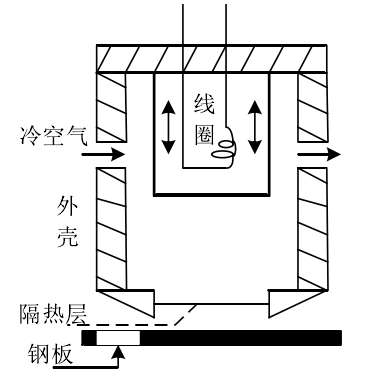
\includegraphics[width=6cm]{c2_eddy.png}
    \caption{电涡流检测原理}
    \label{fig:c2_eddy}
    \end{figure*}

    Helifa等\cite{Helifa2006Detection}设计了一种利用电涡流技术检测裂纹的方法,其方法的目标优化并选择在钢板上检测缺陷的最优电涡流线圈操作参数,首先是确定了使背景信号最小的操作参数来尽量降低背景信号对缺陷信号的干扰,之后通过在真实带缺陷钢板上的实验模拟出了缺陷区域的激励信号并建立了不同形状和大小的缺陷与阻抗平面上的信号的对应关系。其测试流程如图\ref{fig:c2_test_chian}所示:

    \begin{figure*}[!h]
    \centering
    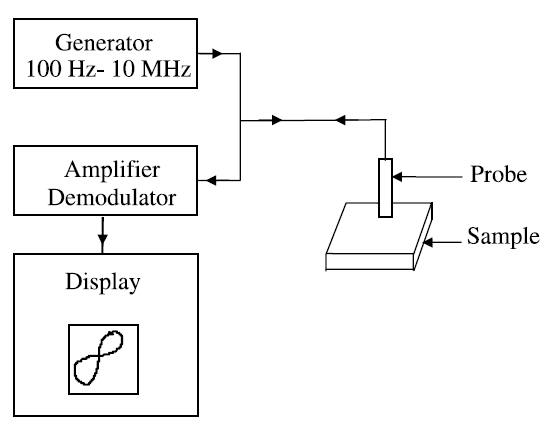
\includegraphics[width=6cm]{c2_test_chain.png}
    \caption{电涡流探伤检测流程}
    \label{fig:c2_test_chian}
    \end{figure*}

    宋凯等\cite{宋凯2015钢管磁特性对涡流检测影响的研究进展}整理并总结了目前使用电涡流技术在钢管无损缺陷检测的应用,阐述了钢管电涡流检测的机理和方法,分析并讨论了影响电涡流检测信号的缺陷漏磁场和缺陷区域畸变的磁导率等磁特性因素,最后总结了当前研究的发展趋势。

    电涡流检测法适用于检测中厚板材表皮与基层的阻流缺陷,该方法需要较大的电流激励才能达到预期的识别效果,因此能耗较大。另外,借助电涡流技术获得热图像必须具备待测板坯保持均匀温度场的前提,且有足够的时间让缺陷充分暴露,毫无疑问这对于高速度、快节奏、强水冷的热轧带钢生产线来讲是无法满足的。而且,使用电涡流检测技术容易受到电涡流探测器本身提离效应的约束,对激励信号的要求也比较高,因此目前国内外在高温连铸坯缺陷检测方面的电涡流检测方法尚未有突破进展。

    1990年,挪威的Elkem首次将红外检测技术用于连铸板坯表面缺陷检测。其系统的工作原理可参考图\ref{fig:c2_infrared},其主要思路是在连铸坯的生产线上装配高频的感应线圈,在满足高频感应的趋肤效应穿透深度小于1mm的情况下,当待检测连铸坯通过感应线圈时在其表面会感生出电流,遇到缺陷区域时,缺陷区域的凹陷或突出部分会产生感应电流,电流路径的延长使单位长度表面上的电能消耗增加,进而使得存在缺陷的连铸坯表面处的局部温度上升,这种局部的温度上升会被四周预装的红外扫描仪获得,从而达到识别钢坯表面缺陷的目的\cite{Vascotto1996High}。 在铸坯表面裂纹和细小孔洞的研究工作中,冈本芳三等\cite{Ooka1988Detection} 学者证明了红外方法的缺陷检测分辨力优于基于X射线检测和超声波探伤的方法。然而,由于缺陷的平均深度、线圈工作频率、感应线圈的宽度、特定的输入电能、钢坯的运动速度、被检钢坯的电性能和热性能以及环境干扰等诸多因素共同决定了缺陷和温升的对应关系,因此红外检测方法对条件依耐性强以及检测稳定性较差,只能局限于离线小范围的应用,难以在环境较为恶劣的热轧带钢生产线大范围推广。

    \begin{figure*}[!h]
    \centering
    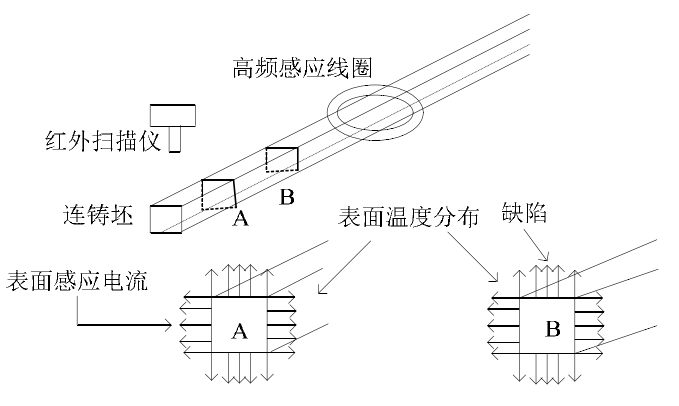
\includegraphics[width=12cm]{c2_infrared.png}
    \caption{红外检测原理}
    \label{fig:c2_infrared}
    \end{figure*}

    漏磁检测法的主要原理是漏磁通密度正比于缺陷体积,所以可以由漏磁通的密度来判断缺陷的大小和种类。在直流磁场中,钢坯被磁化且生成轴向饱和磁场。若钢坯有缺陷,磁通道的改变引起漏磁场的扩散,传感器能把泄露的磁力线检测出来,从而检测出钢坯缺陷的大小。漏磁检测方法的检测原理如图\ref{fig:c2_flux_leakage}。 漏磁检测法除了能检测钢坯表面的缺陷外,还可检测出钢坯内部微小的缺陷,其对于温度要求不高,检测精度高,廉价,但是其不适用于钢坯表面粗糙度的检测,也不能对大量的表面缺陷检测及分类。

    \begin{figure*}[!h]
    \centering
    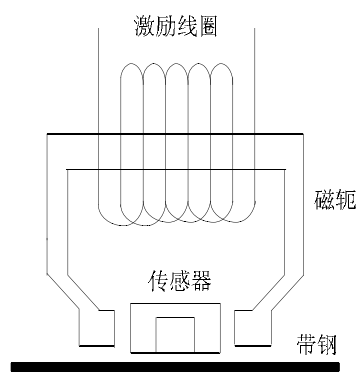
\includegraphics[width=6cm]{c2_flux_leakage.png}
    \caption{漏磁检测原理}
    \label{fig:c2_flux_leakage}
    \end{figure*}

    \section{基于RGB图像的方法}
    \esection{RGB Image based Method}
    相比较于传统无损检测方法,基于RGB图像的方法对钢板自身的物理特性如温度、密度、表面粗糙度等没有要求,并且在检测速度上也有较大优势,这类方法采用CCD摄像机采集钢板表面图像,然后通过图像处理和分析提取出图像特征进行缺陷的提取和分类。

    重庆大学的欧阳奇等\cite{欧阳奇2007高温连铸坯表面缺陷的机器视觉无损检测}针对高温连铸坯表面缺陷无法在线检测的问题,构建了一个连铸坯表面缺陷检测系统,该系统对采集的钢板表面图像进行灰度分析来检测是否存在缺陷,其首先对图像进行平滑滤波以消除噪声,然后对图像进行边缘检测来提取图像边缘,最后对边缘图像进行轮廓搜索将图像上所有的缺陷区域进行标记。

    北京交通大学的王建等\cite{王健2016基于图像分割的钢板表面缺陷识别}采用基于图像分割的方法来检测钢板表面的缺陷,该方法首先对图像进行预处理去除噪声,然后基于图像灰度统计信息的不同,采用了两种图像分割模型,当图像的灰度信息分布均匀时,采用C-V模型对图像进行分割,当图像的灰度信息分布不均匀时,则采用H-T-B模型对图像进行分割,通过这两种模型的组合应用可以对钢板的各类表面缺陷进行检测,获取缺陷区域。其检测的流程图如图\ref{fig:c2_segment_flow_chart} 所示:

    \begin{figure*}[!h]
    \centering
    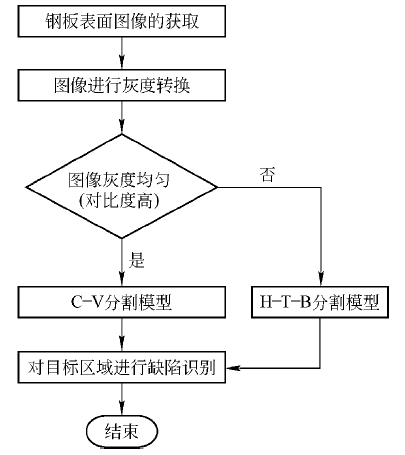
\includegraphics[width=6cm]{c2_segment_flow_chart.png}
    \caption{基于图像分割的缺陷检测流程图}
    \label{fig:c2_segment_flow_chart}
    \end{figure*}

    华中科技大学的刘思等\cite{刘思2011复杂背景下钢板表面缺陷检测的图像增强方法}采用了一种图像增强的办法来提升算法的缺陷检出性能,相较于传统的图像增强算法,该算法能够有效地显示出图像底层的结构特征。该方法首先计算像素的灰度平均值,然后采用均值量化方法将各个像素的灰度值量化为0或者1,接着将量化值输出分解到2个节点中。相比较于直方图均衡化还有分段拉伸,该算法显示出更优的图像增强性能。

    基于RGB图像的方法大部分是在空间域进行操作,主要是提取集合特征、纹理特征、灰度特征还有形状特征等进行缺陷的识别。另外,也有一些学者采用频域变换的方法将图像变换到时域以提取特征,常用的时域变换有Fourier变换、wavelet变换和Gabor变换等。

    中国地质大学的周新星等\cite{周新星2012基于独立成分分析的表面缺陷特征提取与识别方法}采用了一种基于时域变换的方法对钢板表面缺陷进行特征提取和识别,作者首先使用独立成分分析(ICA)和拓扑独立成分分析(TICA)从缺陷集中自适应地估计出基函数和滤波器,这些基函数适应于缺陷图像的特点,然后用于基函数对应的滤波器对钢板图像进行滤波操作,提取滤波响应作为特征向量,最后使用支持向量机对样本进行分类识别。该方法使用的基函数如图\ref{fig:c2_base_function}所示,从左至右依次为ICA 基函数和TICA基函数。该方法建立在对缺陷集无监督学习的基础上,能够自适应地提取缺陷图像的显著特征,且计算简单,可并行处理。该方法所使用的ICA 算法从盲源分离问题发展而来的基于信号高阶统计特性的分析方法,而TICA 则是ICA 的扩展方法。它们用于图像数据时,通过建立观测图像的统计生成模型对图像进行无监督学习,自适应地估计基函数和滤波器,从而用模型中的元素给出图像的表示。

    \begin{figure*}[!h]
    \centering
    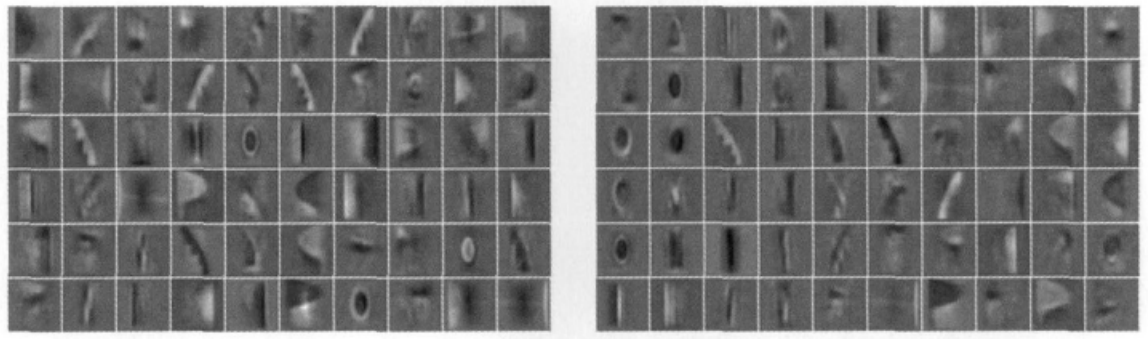
\includegraphics[width=12cm]{c2_base_function.png}
    \caption{缺陷基函数示意图}
    \label{fig:c2_base_function}
    \end{figure*}

    浦项科技大学的Jeon等\cite{Jeon2014Defect}提出了一种基于小波重建的钢板表面缺陷检测算法,该算法首先对钢板图像进行多次独立小波分解,然后对每一层小波分解出的不同分量的信号使用不同的权重加权,然后再将加权后的分量重建成一张新的钢板图像。带权重的二维小波重建的过程如图\ref{fig:c2_wavelet}所示。相比较于原图像,由于在重建的过程中对不同的分量使用了不同的权重,所以重建后的图像更多地保留了原图像的高频信息。接着,该方法对重建后的图像进行双阈值分割,双阈值分割的高低阈值都是根据图像的灰度均值以及标准差来确定的,双阈值分割使用高低阈值分别对图像进行二值化,然后对于每个低阈值分割出的连通区域,若其包含了任一高阈值分割出的连通区域,将其保留,否则抛弃。双阈值分割比一般的阈值分割相比有更高的查全率,并且缺陷轮廓更为完整。分割出缺陷区域后,该方法提取出缺陷的颜色和形态学特征使用支持向量机对缺陷进行分类。

    \begin{figure*}[!h]
    \centering
    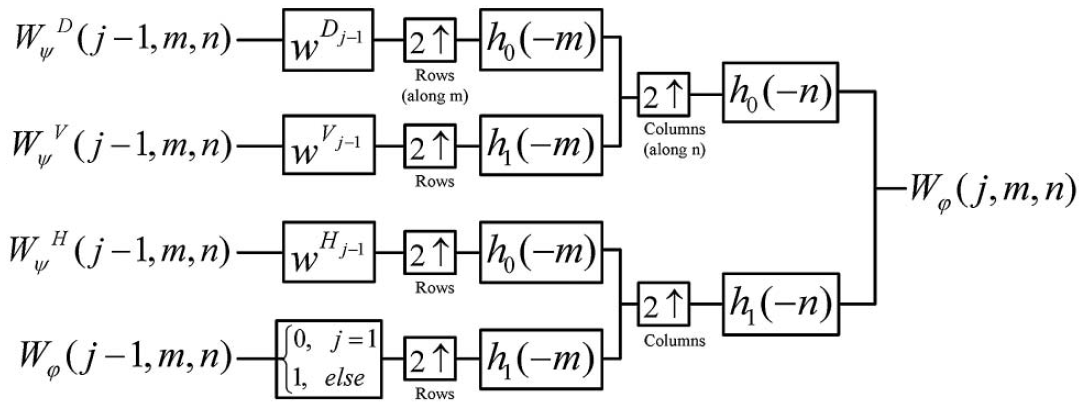
\includegraphics[width=12cm]{c2_wavelet.png}
    \caption{二维加权小波重建示意图}
    \label{fig:c2_wavelet}
    \end{figure*}

    \section{基于深度图像的方法}
    \esection{Depth Image based Method}
    目前深度图像被大量应用于行人检测、步态识别、三维目标识别等领域,但是利用深度图像进行缺陷检测的方法还较少,还没有形成一种典型的流程。相比较于RGB图像,深度图像有先天的优势,首先深度图像不存在RGB图像中反光、模糊、背景复杂等问题,并且由于钢板表面存在氧化铁皮、水膜、黑斑等伪缺陷,使用基于RGB图像的检测方法很难将其检测出来,因为这些伪缺陷在形态和颜色上都与缺陷较为相似,然而这些伪缺陷往往并不具有深度信息,所以在深度图像上往往不会表现出来。

    重庆大学的赵立明等\cite{赵立明2010连铸热坯表面缺陷激光扫描成像三维量化检测方法}设计了一种连铸坯表面缺陷三维量化系统,通过激光扫描成像获取连铸坯表面的深度图像并使用了一些图像处理的技术从深度图像中检测出缺陷。然而作者将深度图像进行灰度化处理,将深度图像当做灰度图像来使用,其检测方法本质上与基于RGB图像的方法类似,并没有真正利用到深度图像的三维特性,与基于RGB图像的方法相比,作者的方法主要还是成像方式不同。

    Zhang等\cite{Zhang2014Continuous}设计了一种钢板表面深度检测系统,作者将光栅投影方法、相位控制方法和时间相位展开方法结合起来检测连铸坯表面的深度信息。文章中显示用该方法检测出的深度图像较为平滑并且对各种缺陷的深度检测适应性较好,该系统的设计如图\ref{fig:c2_zhang}所示,该系统主要包括一台工作站、一个CCD面阵相机和一个数字控制液晶显示投影仪,投影仪能够计算受控结构光,然后通过光学透镜单元将它们投影到目标表面上。该系统主要目标是尽可能准确地测量钢板表面的深度信息,对于提取到深度信息之后,如何利用深度图像提取缺陷,文章中并没有讨论。

    \begin{figure*}[!h]
    \centering
    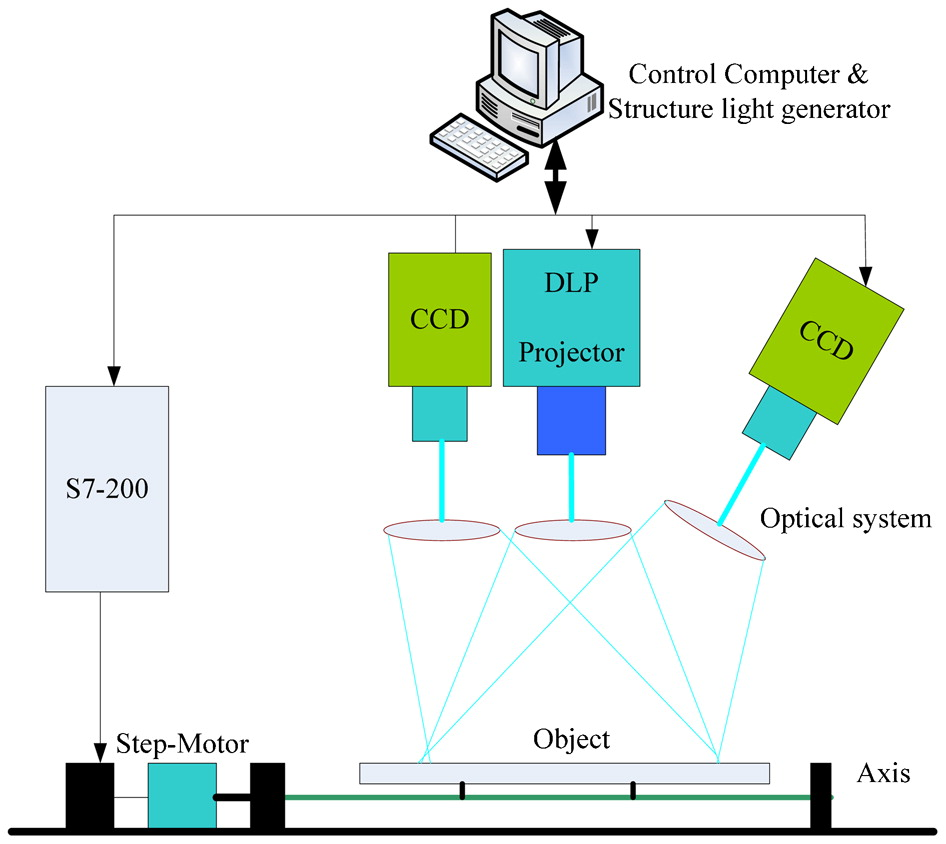
\includegraphics[width=12cm]{c2_zhang.png}
    \caption{系统设计图}
    \label{fig:c2_zhang}
    \end{figure*}

    Landstrom等\cite{Landstrom2012Morphology}提出了一种基于形态学操作的钢板表面裂纹提取算法,作者使用激光三角测量的方法获取了钢板表面深度图像。该方法对三维数据进行了一系列预处理,首先需要确定钢板区域,然后对三维数据进行斜率补偿,接着补齐三维数据中的缺省值,最后使用中值滤波去除噪声,由于一般的三维成像获得的三维数据质量并不高,所以进行这些预处理十分有必要。预处理结束后采用了多种形态学算子来对图像进行形态学操作,接着结合多种形态学操作的计算结果并使用阈值分割的策略获得最终缺陷连通区域,该方法对于裂纹的检测和分类准确率较高,其预处理阶段使用的斜率补偿等方法利用到了深度图像的特点,但是该方法所使用的形态学操作过程主要是针对裂纹这一种缺陷来设计的,对于其他类型的缺陷检出情况如何,作者并没有给出实验结果。

    zhao等\cite{Zhao2014Defect}设计了一个使用成对CCD传感器的连铸坯表面缺陷检测系统,简称DSI,作者使用激光扫描仪和CCD面阵相机同时获取钢板表面的深度图像和灰度图像,其设计的系统如图\ref{fig:c2_DSI_system}所示,该系统使用一个线阵CCD 相机和线阵激光发射器来获取钢板深度数据,另外使用一个面阵CCD相机来获取钢板的灰度图像。作者构建了一个算法将深度图像和灰度图像结合起来检测钢板表面缺陷。为了便于计算,作者首先使用基于互信息的方法将灰度图像和深度图像进行了配准,保证两个图像的像平面是完全对齐的,接着作者根据深度图像中的深度信息定位了一些缺陷种子点,然后根据这些种子点检测除了一些候选的感兴趣区域,接着使用iterative relative fuzzy connectedness 图像分割方法\cite{Udupa2014Body, Udupa1996Disclaimer} 将缺陷区域分割出来。该方法的一大特点就是将深度图像和灰度图像结合起来检测缺陷,由于使用了深度图像,该方法能够有效地抑制伪缺陷例如:氧化铁皮、水膜和黑斑等等,这些伪缺陷对于基于RGB 图像的方法来说往往是一个较大的挑战。另外,该方法不仅能够将缺陷检测出来,还能够准确地提取缺陷部分的轮廓。

    \begin{figure*}[!h]
    \centering
    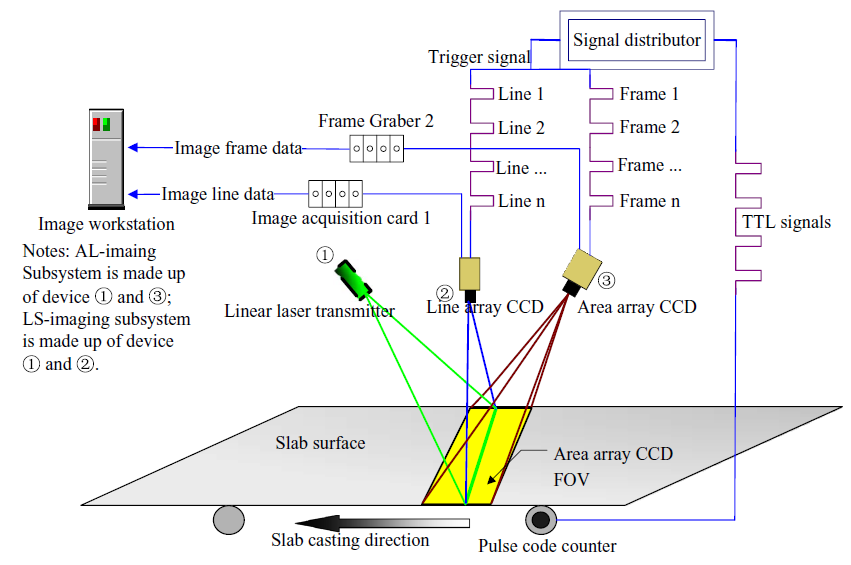
\includegraphics[width=12cm]{c2_DSI_system.png}
    \caption{DSI系统设计图}
    \label{fig:c2_DSI_system}
    \end{figure*}


    \section{本章小结}
    \esection{Brief Summary}
    本章中,主要对现有的连铸坯表面缺陷检测方法进行了整理和总结,现有的连铸坯表面缺陷检测方法主要分为传统无损方法、基于RGB图像的方法和基于深度图像的方法。传统无损方法其主要使用一些钢板的物理特性,通过钢板对电、热、磁等反应的变化来探测缺陷,这些方法往往存在一些局限性,并且方法的实时性不高。基于RGB图像的方法是目前连铸坯表面缺陷检测的研究热点,这些方法主要是使用CCD相机采集钢板灰度图像,然后使用一些图像处理的手段来检测缺陷位置,然而这些算法对于伪缺陷的误检率较高。基于深度图像的方法主要是使用钢板的深度图像来检测缺陷,利用深度信息能够有效地检测出缺陷并排除伪缺陷。

